\documentclass[10pt]{article}
\usepackage[utf8]{inputenc}
\usepackage[T1]{fontenc}
\usepackage{amsmath}
\usepackage{amsfonts}
\usepackage{amssymb}
\usepackage[version=4]{mhchem}
\usepackage{stmaryrd}
\usepackage{graphicx}
\usepackage[export]{adjustbox}
\graphicspath{ {./images/} }
\usepackage{bbold}

\title{2 Structural Specification }

\author{}
\date{}


%New command to display footnote whose markers will always be hidden
\let\svthefootnote\thefootnote
\newcommand\blfootnotetext[1]{%
  \let\thefootnote\relax\footnote{#1}%
  \addtocounter{footnote}{-1}%
  \let\thefootnote\svthefootnote%
}

%Overriding the \footnotetext command to hide the marker if its value is `0`
\let\svfootnotetext\footnotetext
\renewcommand\footnotetext[2][?]{%
  \if\relax#1\relax%
    \ifnum\value{footnote}=0\blfootnotetext{#2}\else\svfootnotetext{#2}\fi%
  \else%
    \if?#1\ifnum\value{footnote}=0\blfootnotetext{#2}\else\svfootnotetext{#2}\fi%
    \else\svfootnotetext[#1]{#2}\fi%
  \fi
}

\begin{document}
\maketitle

The organizational models that follow the organizational centered point of view (e.g., AALAADIN [5], MOISE [9]) usually are composed by two core notions: an Organizational Specification (OS) and an Organizational Entity (OE). An OE is a population of agents functioning under an OS. We can see an OE as an instance of an OS, i.e., agents playing roles defined in the OS (role instance), aggregated in groups instantiated from the OS groups, and behaving as normalized in the OS. Following this trend, a set of agents builds an $\mathrm{OE}$ by adopting an appropriate $\mathrm{OS}$ to easily achieve its purpose. An $\mathcal{MOISE}^{+}$ OS is formed by a Structural Specification (SS), a Functional Specification (FS), and a Deontic Specification (DS). Each of these specifications will be presented in the sequel.

In $\mathcal{MOISE}^{+}$, as in $\mathcal{MOISE}$, three main concepts, roles, role relations, and groups, are be used to build, respectively, the individual, social, and collective structural levels of an organization. Furthermore, the $\mathcal{MOISE}$ original structural dimension is enriched with concepts such as inheritance, compatibility, cardinality, and sub-groups.

Individual level. The individual level is formed by the roles of the organization. A role means a set of constraints that an agent ought to follow when it accepts to enter a group playing that role. Following [2], these constraints are defined in two ways: in relation to other roles (in the collective structural level) and in a deontic relation to global plans (in the functional dimension).

In order to simplify the specification ${ }^{1}$, like in object oriented (OO) terms, there is an inheritance relation among roles [6]. If a role $\rho^{\prime}$ inherits a role $\rho$ (denoted by $\rho \sqsubset \rho^{\prime}$), with $\rho \neq \rho^{\prime}, \rho^{\prime}$ receives some properties from $\rho$, and $\rho^{\prime}$ is a sub-role, or specialization, of $\rho$. In the definition of the role properties presented in the sequence, it will be precisely stated what one specialized role inherits from another role. For example, in the soccer domain, the attacker role has many properties of the player role ( $\left.\rho_{\text {player }} \sqsubset \rho_{\text {attacker }}\right)$. It is also possible to state that a role specializes more than one role, i.e., a role can receive properties from more than one role. The set of all roles are denoted by $\mathcal{R}_{\text {ss }}$.
\footnotetext{${ }^{1}$ Although we will use the term "specification" in the sequence, the $\mathcal{M O I S E}^{+}$could also be used to "describe" an organization.
}

Following this $\mathrm{OO}$ inspiration, we can define an abstract role as a role that can not be played by any agent. It has just a specification purpose. The set of all abstract roles is denotated by $\mathcal{R}_{a b s}\left(\mathcal{R}_{a b s} \subset \mathcal{R}_{s s}\right)$. There is also a special abstract role $\rho_{\text {soc }}$ where $\forall\left(\rho \in \mathcal{R}_{\mathrm{ss}}\right) \rho_{\text {soc }} \sqsubset \rho$, trough the transitivity of $\sqsubset$, all other roles are specializations of it.

Social level. While the inheritance relation does not have a direct effect on the agents behavior, there are other kinds of relations among roles that directly constrain the agents. Those relations are called links [9] and are represented by the predicate $\operatorname{link}\left(\rho_{s}, \rho_{d}, t\right)$ where $\rho_{s}$ is the link source, $\rho_{d}$ is the link destination, and $t \in\{a c q, c o m, a u t\}$ is the link type. In case the link type is acq (acquaintance), the agents playing the source role $\rho_{\mathrm{s}}$ are allowed to have a representation of the agents playing the destination role $\rho_{d}$ ( $\rho_{d}$ agents, in short). In a communication link $(t=c o m)$, the $\rho_{\mathrm{s}}$ agents are allowed to communicate with $\rho_{d}$ agents. In a authority link $(t=a u t)$, the $\rho_{\mathrm{s}}$ agents are allowed to have authority on $\rho_{d}$ agents, i.e., to control them. An authority link implies the existence of a communication link that implies the existence of an acquaintance link:

$$
\begin{aligned}
\operatorname{link}\left(\rho_{s}, \rho_{d}, \text { aut }\right) & \Rightarrow \operatorname{link}\left(\rho_{s}, \rho_{d}, \text { com }\right) \\
\operatorname{link}\left(\rho_{s}, \rho_{d}, \text { com }\right) & \Rightarrow \operatorname{link}\left(\rho_{s}, \rho_{d}, \text { acq }\right)
\end{aligned}
$$

Regarding the inheritance relation, the links follow the rules:

$$
\begin{aligned}
\left(\operatorname{link}\left(\rho_{s}, \rho_{d}, t\right) \wedge \rho_{s} \sqsubset \rho_{s}^{\prime}\right) & \Rightarrow \operatorname{link}\left(\rho_{s}^{\prime}, \rho_{d}, t\right) \\
\left(\operatorname{link}\left(\rho_{s}, \rho_{d}, t\right) \wedge \rho_{d} \sqsubset \rho_{d}^{\prime}\right) & \Rightarrow \operatorname{link}\left(\rho_{s}, \rho_{d}^{\prime}, t\right)
\end{aligned}
$$

For example, if the coach role has authority on the player role $\operatorname{link}\left(\rho_{\text {coach }}, \rho_{\text {player }}\right.$, aut $)$ and player has a sub-role ( $\rho_{\text {player }} \sqsubset \rho_{\text {attacker }}$ ), by Eq. 4, a coach has also authority on attackers. Moreover, a coach is allowed to communicate with players (by Eq. 1) and it is allowed to represent the players (by Eq. 2).

Collective level. The links constrain the agents after they have accepted to play a role. However we should constrain the roles that an agent is allowed to play depending on the roles this agent is currently playing. This compatibility constraint $\rho_{a} \bowtie \rho_{b}$ states that the agents playing the role $\rho_{a}$ are also allowed to play the role $\rho_{b}$ (it is a reflexive and transitive relation). As an example, the team leader role is compatible with the back player role ( $\rho_{\text {leader }} \bowtie \rho_{\text {back }}$ ). If it is not specified that two roles are compatible, by default they are not. Regarding the inheritance, this relation follows the rule

$$
\left(\rho_{a} \bowtie \rho_{b} \wedge \rho_{a} \neq \rho_{b} \wedge \rho_{a} \sqsubset \rho^{\prime}\right) \Rightarrow\left(\rho^{\prime} \bowtie \rho_{b}\right)
$$

Roles can only be played in the collective level, i.e., in a group already created in an $\mathrm{OE}$. We will use the term "group" to mean the instantiated group in an $\mathrm{OE}$ and the term "group specification" to mean the group specified in an OS. Thus, a group must be created from a group specification represented by the tuple

$$
g t={ }_{\text {def }}\left\langle\mathcal{R}, \mathcal{S G}, \mathcal{L}^{\text {intra }}, \mathcal{L}^{\text {inter }}, \mathcal{C}^{\text {intra }}, \mathcal{C}^{\text {inter }}, n p, n g\right\rangle
$$

where $\mathcal{R}$ is the set of not abstract roles that may be played in groups created from $g t$. Once there can be many group specifications, we write the identification of the group
specification as subscript (e.g. $\mathcal{R}_{g t}$ ). The set of possible sub-groups of a group is denoted by $\mathcal{S G}$. If a group specification does not belong to any group specification $\mathcal{S G}$, it is a root group specification.

A group can have intra-group links $\mathcal{L}^{\text {intra }}$ and inter-group links $\mathcal{L}^{\text {inter }}$. The intra-group links state that an agent playing the link source role in a group $g r$ is linked to all agents playing the destination role in the same group $g r$ or in a $g r$ sub-group. The inter-group links state that an agent playing the source role is linked to all agents playing the destination role despite the groups these agents belong to. For example, if there is a link $\operatorname{link}\left(\rho_{\text {student }}, \rho_{\text {teacher }}\right.$, com $) \in$ $\mathcal{L}^{\text {inter }}$, then an agent $\alpha$ playing the role $\rho_{\text {student }}$ is allowed to communicate with the teacher(s) of the groups where it is a student and also with the teachers of any other group, even if $\alpha$ does not belong to these groups.

The roles compatibilities also have a scope. The intra-group compatibilities

\begin{center}
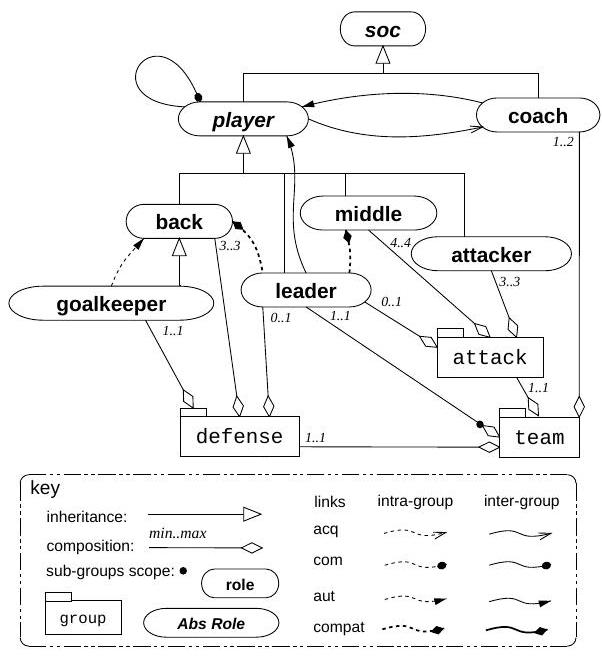
\includegraphics[max width=\textwidth]{2024_01_14_42477cbf96ee593f2d4dg-3}
\end{center}

Fig. 2. Structure of a soccer team $\rho_{a} \bowtie \rho_{b} \in \mathcal{C}^{\text {intra }}$ state that an agent playing the role $\rho_{a}$ in a group $g r$ is allowed to also play the role $\rho_{b}$ in the same group $g r$ or in a $g r$ sub-group. Otherwise, the inter-group compatibilities $\rho_{a} \bowtie \rho_{b} \in \mathcal{C}^{\text {inter }}$ state that an agent playing $\rho_{a}$ in the group $g r_{1}$ is also allowed to play $\rho_{b}$ in other group $g r_{2}\left(g r_{1} \neq g r_{2}\right)$. For instance, an agent can be a teacher in a group and a student in another, but it can not be both in the same group, so it is an inter-group compatibility.

Along with the compatibility, we state that a group is well formed if it respects both the role and sub-groups cardinality. The partial function $n p_{g t}: \mathcal{R}_{g t} \rightarrow \mathbb{N} \times \mathbb{N}$ specifies the number (minimum, maximum) of roles that have to be played in the group, e.g., $n p_{\text {gt }}\left(\rho_{\text {coach }}\right)=(1,2)$ means that $g t$ groups need at least one and no more than two coaches to be well formed. Analogously, the partial function $n g: \mathcal{S G}_{g t} \rightarrow \mathbb{N} \times \mathbb{N}$ specifies the sub-groups cardinality. By default, cardinality pairs are $(0, \infty)$.

For example, the defense soccer team group can be defined as

$$
\begin{gathered}
\text { def }=\left\langle\left\{\rho_{\text {goalkeeper }}, \rho_{\text {back }}, \rho_{\text {leader }}\right\},\{\},\left\{\text { link }\left(\rho_{\text {goalkeeper }}, \rho_{\text {back }}, \text { aut }\right)\right\},\{\},\left\{\rho_{\text {leader }} \bowtie \rho_{\text {back }}\right\},\right. \\
\left.\{\},\left\{\rho_{\text {goalkeeper }} \mapsto(1,1), \rho_{\text {back }} \mapsto(3,3), \rho_{\text {leader }} \mapsto(0,1)\right\},\{\}\right\rangle
\end{gathered}
$$

In this group specification (see Fig. 2), three roles are allowed and any defense group will be well formed if there is one, and only one, agent playing the role goalkeeper, exactly three agents playing backs, and, optionally, one agent playing the leader role. The goalkeeper has authority on the backs and the leader is allowed to be either a back or the goalkeeper, since $\rho_{\text {back }} \sqsubset \rho_{\text {goalkeeper }}$.

Using the recursive definition of group specification, we can specify a team as

$$
\begin{aligned}
\text { team }= & \left\langle\left\{\rho_{\text {coach }}\right\},\{\text { def }, \text { att }\},\{\},\left\{\text { link }\left(\rho_{\text {player }}, \rho_{\text {player }}\right), \text { com }\right),\right. \\
& \text { link } \left.\left.\left.\left.\left(\rho_{\text {leader }}, \rho_{\text {player }}\right), \text { aut }\right), \text { link }\left(\rho_{\text {player }}, \rho_{\text {coach }}\right), \text { acq }\right), \text { link }\left(\rho_{\text {coach }}, \rho_{\text {player }}\right), \text { aut }\right)\right\}, \\
& \left.\{\},\{\},\left\{\rho_{\text {leader }} \mapsto(1,1), \rho_{\text {coach }} \mapsto(1,2)\right\},\{\text { def } \mapsto(1,1), \text { att } \mapsto(1,1)\}\right\rangle
\end{aligned}
$$

A team is well formed if it has one defense group, one attack group, one or two agents playing the coach role, one agent playing the leader role, and the two sub-groups are also well formed. The group att is specified only by the graphical notation presented in the Fig. 2. In this structure, the coach has authority on all players by an inter-group authority link. The players, in any group, can communicate with each other and are allowed to represent the coach. There must be a leader either in the defense or attack group. In the defense group, the leader can also be a back and in the attack group it can be a middle. The leader has authority on all players on all groups, since it has an inter-group authority link on the player role. In this group, an agent ought to belong to just one group because there is no inter-group compatibilities. However, notice that a role may belong to several group specifications (e.g., the leader).

Based on those definitions, the SS of a MAS organization is formed by a set of roles $\left(\mathcal{R}_{s s}\right)$, a set of root group specifications (which may have their sub-groups, e.g. the group specification team), and the inheritance relation ( $\sqsubset$ ) on $\mathcal{R}_{s s}$.

\section*{3 Functional Specification}
The FS in $\mathcal{MOISE}^{+}$ is based on the concepts of missions (a set of global goals²) and global plans (the goals in a structure). These two concepts are assembled in a Social Scheme (SCH) which is essentially a goal decomposition tree where the root is the SCH goal and where the responsibilities for the sub-goals are distributed in missions (see Fig. 3 and Tab. 3 for an example). Each goal may be decomposed in sub-goals through plans which may use three operators:

\begin{itemize}
  \item sequence ",": the plan " $g_{2}=g_{6}, g_{9}$ " means that the goal $g_{2}$ will be achieved if the goal $g_{6}$ is achieved and after that also the goal $g_{9}$ is achieved;
\end{itemize}

\begin{center}
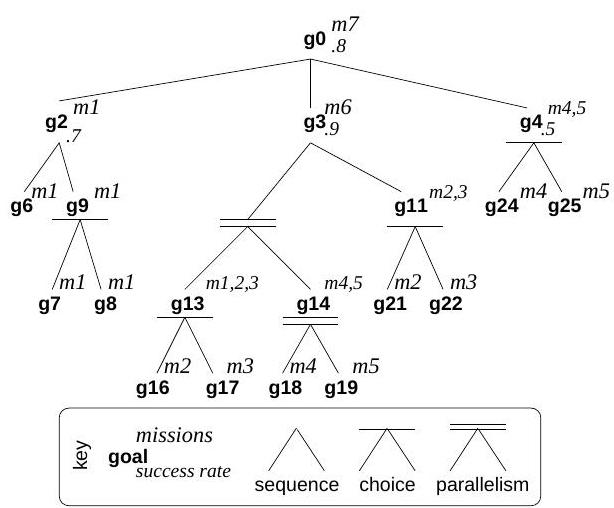
\includegraphics[max width=\textwidth]{2024_01_14_42477cbf96ee593f2d4dg-4}
\end{center}

Fig. 3. An example of Social Scheme to score a soccer goal
- choice "|": the plan " $g_{9}=g_{7} \mid g_{8}$ " means that the goal $g_{9}$ will be achieved if one, and only one, of the goals $g_{7}$ or $g_{8}$ is achieved; and
- parallelism " $\|$ ": the plan " $g_{10}=g_{13} \| g_{14}$ " means that the goal $g_{10}$ will be achieved if both $g_{13}$ and $g_{14}$ are achieved, but they can be achieved in parallel.
\footnotetext{${ }^{2}$ Regarding the terminology proposed in [3], these goals are collective goals and not social goals. Since we have taken an organizational centered approach, it is not possible to concept the social goal which depends on the agents internal mental state.
}

It is also useful to add a certainty success degree in a plan. For example, considering the plan " $g_{2}=g_{6},\left(g_{7} \mid g_{8}\right)$ ", there may be a environment where the achievement of $g_{6}$ followed by the achievement of $g_{7}$ or $g_{8}$ does not imply the achievement of $g_{2}$. Usually the achievement of the plan right side implies the achievement of the plan goal $g_{2}$, but in some contexts this may not happen. Thus, the plan has a success degree that is continually updated from its performance success. This value is denoted by a subscript on the $=$. For example, the plan " $g_{2}={ }_{0.85} g_{6},\left(g_{7} \mid g_{8}\right)$ "

achieves $g_{2}$ with $85 \%$ of certainty.

In a SCH, a mission is a set of coherent goals that an agent can commit to. For instance, in the SCH of the Fig. 3 , the mission $m_{2}$ has two goals $\left\{g_{16}, g_{21}\right\}$, thus, the agent that accepts $m_{2}$ is committed to the goals $g_{16}$ and $g_{21}$. More precisely, if an agent $\alpha$ accepts a mission $m_{i}$, it commits to all goals of $m_{i}\left(g_{j} \in m_{i}\right)$ and $\alpha$ will try to achieve a $g_{j}$ goal only when the precondition goal for $g_{j}$ is already achieved. This precondition goal is inferred from the sequence operator (e.g.: the goal $g_{16}$ of the Fig. 3 can be tried only after $g_{2}$ is already achieved; $g_{21}$ can be tried only after $g_{10}$ is achieved).

A Social Scheme is represented by a tuple $\langle\mathcal{G}, \mathcal{M}, \mathcal{P}$, mo, $n m\rangle$ where $\mathcal{G}$ is the set of global goal; $\mathcal{M}$ is the set of mission labels; $\mathcal{P}$ is the set of plans that builds the tree structure; $m o: \mathcal{M} \rightarrow \mathbb{P}(\mathcal{G})$ is a function that specifies the mission set of goals; and $n m: \mathcal{M} \rightarrow \mathbb{N} \times \mathbb{N}$ specifies the number (minimum, maximum) of agents that have to commit to each mission in order to say the SCH is well formed, by default, this pair is $(1, \infty)$, i.e., one or more agents can commit to the mission.

For example, a SCH to score a soccer-goal ( $s g$ ) could be (see Fig. 3):

$$
\begin{aligned}
s g= & \left\langle\left\{g_{0}, \ldots, g_{25}\right\},\left\{m_{1}, \ldots, m_{7}\right\},\left\{“ g_{0}=.8 g_{2}, g_{3}, g_{4} \text { ”“" } g_{2}=.7 g_{6}, g_{9}\right),, \ldots\right\}, \\
& \left\{m_{1} \mapsto\left\{g_{2}, g_{6}, g_{7}, g_{8}, g_{13}\right\}, m_{2} \mapsto\left\{g_{13}, g_{16}, g_{11}, g_{24}\right\}, \ldots, m_{7} \mapsto\left\{g_{0}\right\}\right\}, \\
& \left.\left\{m_{1} \mapsto(1,4), m_{2} \mapsto(1,1), m_{3} \mapsto(1,1), \ldots\right\}\right\rangle
\end{aligned}
$$

This SCH is well formed if from one to four agents have committed to $m_{1}$ and one, and at most one, agent has committed to the other missions. The agent that will commit to the mission $m_{7}$ is the very agent that has the permission to create this SCH and to start its execution, since the $m_{7}$ is the $s g$ root goal.

It is also possible to define a preference order among the missions. If the FS includes $m_{1} \prec m_{2}$, then the mission $m_{1}$ has a social preference on the mission $m_{2}$. If there is a moment when an agent is permitted to $m_{1}$ and also $m_{2}$, it has to prioritize the execution of $m_{1}$. Since $m_{1}$ and $m_{2}$ could belong to different SCHs, one can use this operator to specify the preferences among SCHs. For example, if $m_{1}$ is the root mission of the SCH for an attack through one side of the field $(\mathrm{sg})$ and $m_{2}$ is the root of other SCH for the substitution of a player, then $m_{1} \prec m_{2}$ means that the $s g$ must be prioritized.

To sum up, the FS is a set of several SCHs and mission preferences which describes how a MAS usually achieves its global goals, i.e., how these goals are decomposed by plans and distributed to the agents by missions. The FS evolve either by the MAS designer who specifies its expertise in a SCH form or by the agents themselves that store their (best) past solutions (as an enterprise does through its "procedures manual").

\section*{4 Deontic Specification}
The FS and SS of a MAS, as described in Sec. 2 and Sec. 3, can be defined independently. However, our view of the organization effects on a MAS suggests a kind of relation among them (Fig. 1). So in $\mathcal{M O I S E}{ }^{+}$this relation is specified in the individual level as permissions and obligations of a role on a mission.

A permission $\operatorname{per}(\rho, m, t c)$ states that an agent playing the role $\rho$ is allowed to commit to the mission $m$, and $t c$ is a time constraint on the permission, i.e., it specifies a set of periods during which this permission is valid, e.g.: every day/all hours, for Sundays/from $14 \mathrm{~h}$ to $16 \mathrm{~h}$, for the first month day/all hours. In order to save space, the language for specifying the $t c$ is not described here (it is based on the definitions presented in [1]). Any is a tc set that means "every day/all hours". Furthermore, an obligation $o b l(\rho, m, t c)$ states that an agent playing $\rho$ ought to commit to $m$ in the periods listed in $t c$. These two predicates have the following properties: if an agent is obligated to a mission it is also permitted to this mission; and deontic relations are inherited:

$$
\begin{aligned}
\operatorname{obl}(\rho, m, t c) & \Rightarrow \operatorname{per}(\rho, m, t c) \\
\operatorname{obl}(\rho, m, t c) \wedge \rho \sqsubset \rho^{\prime} & \Rightarrow \operatorname{obl}\left(\rho^{\prime}, m, t c\right) \\
\operatorname{per}(\rho, m, t c) \wedge \rho \sqsubset \rho^{\prime} & \Rightarrow \operatorname{per}\left(\rho^{\prime}, m, t c\right)
\end{aligned}
$$

For example, a team deontic specification could be:

$$
\begin{aligned}
& \left\{\operatorname{per}\left(\rho_{\text {goalkeeper }}, m_{7}, \text { Any }\right)\right\},\left\{\text { obl }\left(\rho_{\text {goalkeeper }}, m_{1}, \text { Any }\right),\right. \\
& \text { obl }\left(\rho_{\text {back }}, m_{1}, \text { Any }\right), \text { obl }\left(\rho_{\text {leader }}, m_{6}, \text { Any }\right), \text { obl }\left(\rho_{\text {middle }}, m_{2}, \text { Any }\right), \\
& \text { obl } \left.\left.\left(\rho_{\text {middle }}, m_{3}, \text { Any }\right), \text { obl }\left(\rho_{\text {attacker }}, m_{4}, \text { Any }\right), \text { obl }\left(\rho_{\text {attacker }}, m_{5}, \text { Any }\right)\right\}\right\rangle
\end{aligned}
$$

In our example, the goalkeeper can decide that the SCH $s g$ will be performed. The goalkeeper has this right due its permission for the $s g$ mission root (Fig. 3). Once the SCH is created, other agents (playing $\rho_{\text {back }}, \rho_{\text {leader }}, \ldots$ ) are obligated to participate in this SCH. These other agents ought to pursue their sg goals just in the moment allowed by this SCH. For instance, the middle agent $\alpha$ that accepts the mission $m_{2}$ will try to get the ball $\left(g_{16}\right)$ only after the ball is in the middle field ( $g_{2}$ was achieved).


\end{document}